\subsubsection{Luminance and contrast}

To transform the stimulus patch $\patchmatrix$ to the patch of PING networks in V1, we apply the lattice of size $n \times n$, such that each oscillatory network contains a field of $m \times m$ pixels. An example of the resulting lattice is displayed in Figure \ref{fig:llc-lattice-example}.


\begin{figure}[!htp]
    \centering
    \begin{subfigure}[t]{0.4\textwidth}
        \centering
        \newcommand{\splw}{\textwidth}
\newcommand{\splh}{\splw}

\newcommand{\splnrverticallines}{11}
\newcommand{\splverticalinterval}{0.08333} % 1 / (splnrverticallines + 1)

\newcommand{\splnrhorizontallines}{11}
\newcommand{\splhorizontalinterval}{0.08333}

\begin{tikzpicture}[
    cline/.style = {very thick, color-one},
]
    \begin{scope}
        \node[anchor=south west,inner sep=0] at (0,0) {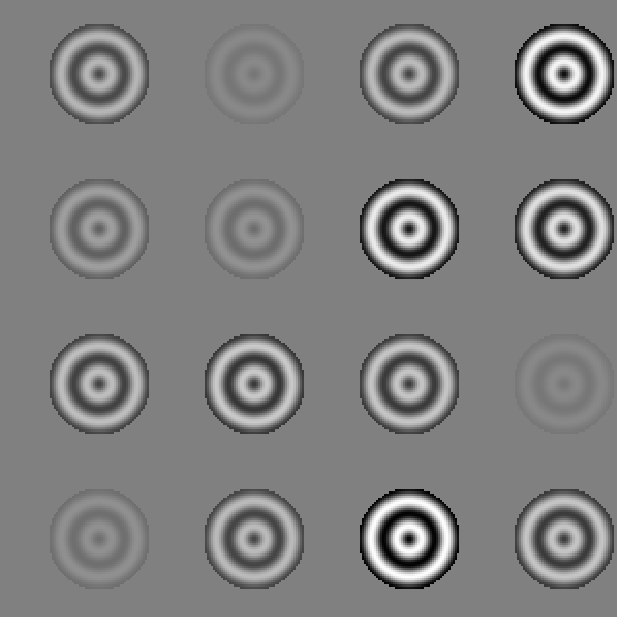
\includegraphics[width=\splw]{src/assets/images/stimulus-patch-lattice.png}};
        
        % vertical
        \foreach \i in {1, 2, ..., \splnrverticallines}{
            \draw[cline] (\i * \splverticalinterval * \splw, 0) -- (\i * \splverticalinterval * \splw, \splh) {};
        }
        
        % horizontal
        \foreach \i in {1, 2, ..., \splnrverticallines}{
            \draw[cline] (0, \i * \splhorizontalinterval * \splh) -- (\splw, \i * \splhorizontalinterval * \splh) {};
        }

    \end{scope}
\end{tikzpicture}
        \caption{A $12 \times 12$ lattice applied to a patch.}
        \label{fig:llc-lattice-example}
    \end{subfigure}
    \hspace{0.06\textwidth}
    \begin{subfigure}[t]{0.4\textwidth}
        \centering
        
\includegraphics[width=\textwidth]{src/assets/images/local-contrast.png}
        \caption{Local contrasts of the patch in Figure \ref{fig:llc-lattice-example}: $0$ (black) $\to$ $1$ (white).}
        \label{fig:llc-local-contrast-example}
    \end{subfigure}
    \caption[Patch lattice and local contrast]{The lattice of a patch and its vertices' local contrasts. The parameters with which the patch was generated: $\diam = 53, \anndistscale = 1.6, \contrange = 1, \figeccdg = 11^\circ, \patchsizedg = 3^\circ$; the rest of the parameters are equal to the ones used in Figure \ref{fig:full-stimulus-example}.}
    \label{fig:lattice-local-contrast-example}
\end{figure}


Let $V_\ping$ be the set containing the PING networks. Let $\pix: V_\ping \to (\mathbb{Z}_+)^{2 \times m^2}$ be a function mapping a network to the set of all $m^2$ pixel coordinates it contains.
For each network $v \in V_\ping$, a local contrast $\LC: V \to \mathbb{R}$ is the weighted root-mean-squared (RMS) contrast defined as follows \cite{Frazor2006}:
\begin{equation}
    \LC_v = \sqrt{
        \frac{
            \sum_{(i, j) \in \pix(v)} \weight_{v, (i, j)} \frac{(\patchmatrix_{i, j} - \overline{\fullmatrix})^2}{\overline{\fullmatrix}}
        }{
            \sum_{(i, j) \in \pix(v)} \weight_{v, (i, j)}
        }
    },
\end{equation}
where $\overline{\fullmatrix}$ is the mean over all luminance values in $\fullmatrix$, and $\weight: V_\ping, \mathbb{N}^2 \to \mathbb{R}$ is the weight of a pixel with respect to a network, as shown in Equation (\ref{eq:weight-pixel-network}). An example of a local contrast matrix can be seen in Figure \ref{fig:llc-local-contrast-example}.

To define that weight, one first needs to complete a number of steps.
Let $\centr : V_\ping \to \mathbb{R}_+^2$ be the function mapping a particular PING network in the patch to the location of its center. As the center of the gaze (fovea) coincides with the center of the stimulus, the eccentricity $\ecc: V_\ping \to \mathbb{R}_+$ in degrees for a network $v \in V_\ping$ is
\begin{equation}
    \ecc_{v} = \frac{1}{\atopix} \cdot \left\| \left( \frac{\fullwidth}{2}, \frac{\fullheight}{2}   \right), \patchstart + \centr(v) \right\|.
\end{equation}

Let $\slope \in \mathbb{R}$ be the slope, the ratio of receptive field diameter to eccentricity, and $\intercept \in \mathbb{R}$ - the intercept \cite{MaryamPLACEHOLDER}, \cite{Freeman2011}.
Let $\diamRF_{\min} \in \mathbb{R}_+$ be smallest allowed diameter of the receptive field.
Then, the diameter of the receptive field $\diamRF \in \mathbb{R}$ of $v$ is 
\begin{equation}
    \diamRF_v = \max{( \slope \cdot \ecc_v + \intercept, \ \diamRF_{\min} )}.
\end{equation}

Let $\stdrf: V_\ping \to \mathbb{R}$ be the standard deviation of the receptive field diameter of a Gaussian beam \todo{why do we consider it a Gaussian beam? Email Mario}. It can be obtained by utilizing the full width at half maximum $\fwhm: V_\ping \to \mathbb{R}$ in the following way \cite{MaryamPLACEHOLDER}:
\begin{equation}
    \begin{cases}
        \fwhm_v = \sqrt{\frac{\ln(2)}{2}} \cdot \diamRF_v \\
        \fwhm_v = 2 \sqrt{2 \ln(2)} \cdot \stdrf_v
    \end{cases}
    \Rightarrow 
    \stdrf_v = \frac{1}{4} \diamRF_v.
\end{equation}

Having derived the standard deviation, the weight of the pixel $i, j \in \{ 0, 1, \cdots, \patchsize - 1 \}$ with respect to a PING network $v$ can be defined at last. This value is specific to each network as it reflects its unique receptive field modeled with an isotropic 2D Gaussian function \cite{MaryamPLACEHOLDER}:
\begin{equation}
    \weight_{v, (i, j)} = \exp \left(
        -\frac{ \frac{1}{\atopix} \cdot \| (i, j), \ \centr(v) \|}{ 2 \stdrf_v^2 }
    \right).
    \label{eq:weight-pixel-network}
\end{equation}